% Copyright 2004 by Till Tantau <tantau@users.sourceforge.net>.
%
% In principle, this file can be redistributed and/or modified under
% the terms of the GNU Public License, version 2.
%
% However, this file is supposed to be a template to be modified
% for your own needs. For this reason, if you use this file as a
% template and not specifically distribute it as part of a another
% package/program, I grant the extra permission to freely copy and
% modify this file as you see fit and even to delete this copyright
% notice. 

\PassOptionsToPackage{usenames,dvipsnames}{xcolor}

\documentclass[compress]{beamer}

\usepackage{amsmath}
\usepackage{xcolor}
\usepackage{cancel}
\newcommand\Ccancel[2][black]{\renewcommand\CancelColor{\color{#1}}\xcancel{#2}}

\usepackage{tikz}
\usetikzlibrary{arrows,shapes,chains,fit,calc,patterns}
\usepackage{graphicx}
\usepackage{varwidth}

\usepackage{multirow} 

\usepackage[super]{nth}

%\usepackage{listings}
%\usepackage{minted}
%\usemintedstyle{colorful}

%\usepackage{pgfpages}
%\setbeameroption{show notes}

% TODO Add personal theme
\usetheme{default}


\setbeamertemplate{footline}[frame number]

\newcommand{\smallnode}[1]{\begin{varwidth}{0.4cm}\scalebox{0.8}{\hspace{-0.2cm}#1}\end{varwidth}}
\newcommand{\fun}[1]{\mathtt{{#1}}}


\title{Verifying Recursive Program via Source-to-Source Program Transformation}
\author{Presenter: Chiao~Hsieh\inst{1,2}}

\institute{
  \inst{1}
  Institute of Information Science, 
  Academia Sinica
  \and
  \inst{2}
  Graduate Institute of Electrical Engineering,
  National Taiwan University
}

\date{July 3, 2015}

% If you have a file called "university-logo-filename.xxx", where xxx
% is a graphic format that can be processed by latex or pdflatex,
% resp., then you can add a logo as follows:

% \pgfdeclareimage[height=0.5cm]{university-logo}{university-logo-filename}
% \logo{\pgfuseimage{university-logo}}

% Delete this, if you do not want the table of contents to pop up at
% the beginning of each subsection:
\AtBeginSection[]
{
  \begin{frame}<beamer>{Outline}
    \tableofcontents[currentsection, hideallsubsections]
  \end{frame}
}

%\includeonly{tex/approx}

% Let's get started
\begin{document}

\begin{frame}
  \titlepage
\end{frame}

\begin{frame}{Previous Works}
\begin{itemize}
  \item Verifying Recursive Programs Using Intraprocedural Analyzers
  \begin{itemize}
    \item The 21th International Static Analysis Symposium~(SAS 2014)
    \item Author: Yu-Fang Chen, Chiao Hsieh, Ming-Hsien Tsai, Bow-Yaw Wang, Farn Wang
  \end{itemize}
  \vfill
  \item CPArec: Verifying Recursive Programs via Source-to-Source Program Transformation
  \begin{itemize}
    \item 21st International Conference on Tools and Algorithms
          for the Construction and Analysis of Systems~(TACAS 2015)
    \item Contribution on Software Verification Competition
    \item Author: Yu-Fang Chen, Chiao Hsieh, Ming-Hsien Tsai, Bow-Yaw Wang, Farn Wang
  \end{itemize}
\end{itemize}
\end{frame}

\begin{frame}{Outline}
  \tableofcontents[hideallsubsections]
  % You might wish to add the option [pausesections]
\end{frame}

% Section and subsections will appear in the presentation overview
% and table of contents.
\section{Overview}
\stepcounter{subsection}

\def \unit {0.8mm}
\newsavebox{\pokerface}
\savebox{\pokerface}
{
  \begin{tikzpicture}
    \node [inner sep=0, text width=20*\unit]
    {
\includegraphics[width=\textwidth]{img/pokerface_clean}};
  \end{tikzpicture}
}

\begin{frame}{Overview}

\begin{overlayarea}{\textwidth}{.1\textheight}
   \only<1>{Powerful existing analyzers for recursion-free program
          }\only<2>{Limited or no support for recursion
          }\only<3>{Approximate and Refine via {\color{red}syntactic transformation}
          }\only<4>{Guess \& Check
          }\only<5-7>{Progress Iteratively}
    \begin{itemize}
      \item \only<1>{Years of hard work
            }\only<2>{However, hard for us to modify their work
            }\only<3>{Able to treat the analyzer as a black-box
            }\only<4>{Achieved by transformation and output from \colorbox{black}{\color{white}Analyzer}
            }\only<5>{More accurate
            }\only<6-7>{More and more accurate}
    \end{itemize}
\end{overlayarea}

\center
\begin{tikzpicture}[
  x=1*\unit, y=1*\unit,
  approx/.style={draw=black,pattern color=OliveGreen, pattern=north east lines},
  result_node/.style={draw, rounded rectangle, minimum width=20*\unit},
  analyzer/.style={inner sep=0, diamond, aspect=2, fill=black, text=white},
  every edge/.style={draw, ->, >=latex', thick},
  cross_out/.style = {red, pos=0.5, auto=false, cross out, -, draw, thick}
  ]

  \path[use as bounding box] (-66,-40) rectangle (66,40);
  \node [result_node, text=green] (pass) at (54, 20) {PASS};
  \node [result_node, text=red] (error) at (54, -20) {ERROR};

  \node<1-2> [analyzer, label=above:{Black-box}, label=below:{CPAchecker}] (basic_analyzer) at (24, 0){Analyzer};
  \node<3->[analyzer] (analyzer_under) at (24,-20) {Analyzer};
  \node<3>[analyzer] (analyzer_over)  at (24, 20) {Analyzer};
  \node<4->[analyzer, fill=Gray](check) at (analyzer_over) {Check};

  \node<1>[draw=none, minimum width=30*\unit, minimum height=30*\unit, label=above:{Recursion-free program}]
    (creeper) at (-54, 0){};
  \filldraw<1>[approx, even odd rule]
    ($ (creeper) + (-12, -12) $) rectangle ($ (creeper) + (12, 12) $)
    ($ (creeper) + (-9, 0) $) rectangle ($ (creeper) + (-3, 6) $)
    ($ (creeper) + (3, 0) $) rectangle ($ (creeper) + (9, 6) $)
    ($ (creeper) + (-6, -12) $)--($ (creeper) + (-3, -12) $)
    --($ (creeper) + (-3, -9) $) --($ (creeper) + (3, -9) $)
    --($ (creeper) + (3, -12) $) --($ (creeper) + (6, -12) $)
    --($ (creeper) + (6, -3) $) --($ (creeper) + (3, -3) $)
    --($ (creeper) + (3, 0) $) --($ (creeper) + (-3, 0) $)
    --($ (creeper) + (-3, -3) $) --($ (creeper) + (-6, -3) $)--cycle;

  \draw<2-> [approx, draw=none] % draw background
    ($ (creeper) + (-10, -14) $) rectangle ($ (creeper) + (10, 14) $);
  \node<2-> [label=above:{Recursive program}] (poker) at (creeper) {\usebox{\pokerface}};

  \node<3-> (poker_over) at (-10, 20){\usebox{\pokerface}};
  \draw<3-4> [approx]
    ($ (poker_over) + (-12, -18) $) rectangle ($ (poker_over) + (12, 18) $);
  \draw<5> [approx]
    ($ (poker_over) + (-12, -6) $) -- ($ (poker_over) + (-6, -6) $)
    -- ($ (poker_over) + (-6, -12) $) -- ($ (poker_over) + (0, -12) $)
    -- ($ (poker_over) + (0, -18) $) -- ($ (poker_over) + (6, -18) $)
    -- ($ (poker_over) + (6, -12) $) -- ($ (poker_over) + (12, -12) $)
    -- ($ (poker_over) + (12, 12) $) -- ($ (poker_over) + (6, 12) $)
    -- ($ (poker_over) + (6, 18) $) -- ($ (poker_over) + (-12, 18) $)
    -- cycle;
  \draw<6> [approx]
    ($ (poker_over) + (-12, -3) $) -- ($ (poker_over) + (-9, -3) $)
    -- ($ (poker_over) + (-9, -6) $) -- ($ (poker_over) + (-6, -6) $)
    -- ($ (poker_over) + (-6, -9) $) -- ($ (poker_over) + (0, -9) $)
    -- ($ (poker_over) + (0, -15) $) -- ($ (poker_over) + (3, -15) $)
    -- ($ (poker_over) + (3, -9) $) -- ($ (poker_over) + (9, -9) $)
    -- ($ (poker_over) + (9, -6) $) -- ($ (poker_over) + (12, -6) $)
    -- ($ (poker_over) + (12, 6) $) -- ($ (poker_over) + (9, 6) $)
    -- ($ (poker_over) + (9, 12) $) -- ($ (poker_over) + (6, 12) $)
    -- ($ (poker_over) + (6, 15) $) -- ($ (poker_over) + (-9, 15) $)
    -- ($ (poker_over) + (-9, 12) $)-- ($ (poker_over) + (-12, 12) $)
    -- cycle;
  \draw<7-> [approx]
    ($ (poker_over) + (-10.5, -3) $) -- ($ (poker_over) + (-9, -3) $)
    -- ($ (poker_over) + (-9, -4.5) $) -- ($ (poker_over) + (-7.5, -4.5) $)
    -- ($ (poker_over) + (-7.5, -6) $) -- ($ (poker_over) + (-6, -6) $)
    -- ($ (poker_over) + (-6, -7.5) $) -- ($ (poker_over) + (-4.5, -7.5) $)
    -- ($ (poker_over) + (-4.5, -9) $) -- ($ (poker_over) + (0, -9) $)
    -- ($ (poker_over) + (0, -12) $) -- ($ (poker_over) + (1.5, -12) $)
    -- ($ (poker_over) + (1.5, -15) $) -- ($ (poker_over) + (3, -15) $)
    -- ($ (poker_over) + (3, -9) $) -- ($ (poker_over) + (7.5, -9) $)
    -- ($ (poker_over) + (7.5, -7.5) $) -- ($ (poker_over) + (9, -7.5) $)
    -- ($ (poker_over) + (9, -6) $) -- ($ (poker_over) + (10.5, -6) $)
    -- ($ (poker_over) + (10.5, 6) $) -- ($ (poker_over) + (9, 6) $)
    -- ($ (poker_over) + (9, 9) $) -- ($ (poker_over) + (7.5, 9) $)
    -- ($ (poker_over) + (7.5, 10.5) $) -- ($ (poker_over) + (6, 10.5) $)
    -- ($ (poker_over) + (6, 12) $) -- ($ (poker_over) + (4.5, 12) $)
    -- ($ (poker_over) + (4.5, 13.5) $) -- ($ (poker_over) + (1.5, 13.5) $)
    -- ($ (poker_over) + (1.5, 15) $) -- ($ (poker_over) + (-7.5, 15) $)
    -- ($ (poker_over) + (-7.5, 13.5) $) -- ($ (poker_over) + (-9, 13.5) $)
    -- ($ (poker_over) + (-9, 12) $)-- ($ (poker_over) + (-10.5, 12) $)
    -- cycle;

  \node<3-> [label=below:{Recursion-free}] (poker_under) at (-10, -20){\usebox{\pokerface}};
  \draw<3-4> [approx]
    ($ (poker_under) + (-6, -5) $) rectangle ($ (poker_under) + (6, 7) $);
  \draw<5> [approx]
    ($ (poker_under) + (-6, -5) $) -- ($ (poker_under) + (6, -5) $)
    -- ($ (poker_under) + (6, 7) $) -- ($ (poker_under) + (0, 7) $)
    -- ($ (poker_under) + (0, 13) $) -- ($ (poker_under) + (-6, 13) $)
    -- cycle;
  \draw<6> [approx]
    ($ (poker_under) + (-9, 1) $)  -- ($ (poker_under) + (-6, 1) $)
    -- ($ (poker_under) + (-6, -5) $) -- ($ (poker_under) + (0, -5) $)
    -- ($ (poker_under) + (0, -8) $) -- ($ (poker_under) + (3, -8) $)
    -- ($ (poker_under) + (3, -5) $) -- ($ (poker_under) + (6, -5) $)
    -- ($ (poker_under) + (6, -2) $) -- ($ (poker_under) + (9, -2) $)
    -- ($ (poker_under) + (9, 4) $) -- ($ (poker_under) + (6, 4) $)
    -- ($ (poker_under) + (6, 7) $) -- ($ (poker_under) + (3, 7) $)
    -- ($ (poker_under) + (3, 10) $) -- ($ (poker_under) + (0, 10) $)
    -- ($ (poker_under) + (0, 13) $) -- ($ (poker_under) + (-6, 13) $)
    -- ($ (poker_under) + (-6, 10) $) -- ($ (poker_under) + (-9, 10) $)
    -- cycle;
  \draw<7-> [approx]
    ($ (poker_under) + (-9, -0.5) $)  -- ($ (poker_under) + (-7.5, -0.5) $)
    -- ($ (poker_under) + (-7.5, -3.5) $) -- ($ (poker_under) + (-6, -3.5) $)
    -- ($ (poker_under) + (-6, -5) $) -- ($ (poker_under) + (-4.5, -5) $)
    -- ($ (poker_under) + (-4.5, -6.5) $) -- ($ (poker_under) + (-1.5, -6.5) $)
    -- ($ (poker_under) + (-1.5, -8) $) -- ($ (poker_under) + (4.5, -8) $)
    -- ($ (poker_under) + (4.5, -6.5) $) -- ($ (poker_under) + (7.5, -6.5) $)
    -- ($ (poker_under) + (7.5, -3.5) $) -- ($ (poker_under) + (9, -3.5) $)
    -- ($ (poker_under) + (9, 4) $) -- ($ (poker_under) + (7.5, 4) $)
    -- ($ (poker_under) + (7.5, 7) $) -- ($ (poker_under) + (6, 7) $)
    -- ($ (poker_under) + (6, 8.5) $) -- ($ (poker_under) + (4.5, 8.5) $)
    -- ($ (poker_under) + (4.5, 10) $) -- ($ (poker_under) + (3, 10) $)
    -- ($ (poker_under) + (3, 11.5) $) -- ($ (poker_under) + (0, 11.5) $)
    -- ($ (poker_under) + (0, 13) $) -- ($ (poker_under) + (-6, 13) $)
    -- ($ (poker_under) + (-6, 11.5) $) -- ($ (poker_under) + (-7.5, 11.5) $)
    -- ($ (poker_under) + (-7.5, 10) $) -- ($ (poker_under) + (-9, 10) $)
    -- cycle;

%% Draw edges
  \path<1>
    (creeper) edge (basic_analyzer.west);
  \path<2>
    (poker) edge node [draw, cross_out, red] {} (basic_analyzer.west);
  \path<1-2>
    (basic_analyzer.east) edge (error) edge (pass);
  \path<3->
    (poker) edge node[anchor=north,sloped] (under-approx) {Under-approx.}(poker_under)
    (poker_under) edge (analyzer_under)
    (analyzer_under.east) edge node[anchor=north,sloped]{Error} (error)
    ;
  \path<3>
    (poker_over)  edge (analyzer_over)
    (analyzer_over.east) edge node[anchor=south,sloped]{Pass} (pass)
    (analyzer_over.north) edge[bend right] node[anchor=south,sloped]{\only<7>{\Ccancel[red]}{Error, Refine}} (poker_over)
    (analyzer_under.north) edge[bend right] node[anchor=south,sloped]{Pass, Refine} (poker_under)
    ;
  \path<3-4>
    (poker) edge node[anchor=south,sloped] (over-approx) {\only<4>{\Ccancel[red]}{Over-approx.}}(poker_over)
    ;
  \path<4->
    (analyzer_under.north) edge node[anchor=west]{Pass, \only<4>{\color{red}}Compute over-approx.} (poker_over)
    (poker_over) edge (check)
    (check) edge node[anchor=south]{Pass} (pass)
    (check) edge node[anchor=west]{Error, Refine} (poker_under)
    ;
\end{tikzpicture}
\end{frame}

\begin{frame}{Overview}
\tikzstyle{decision} = [diamond, aspect=2, draw, align=center]
\tikzstyle{data} = [draw,trapezium,trapezium left angle=70,trapezium right angle=-70,minimum height=0.6cm]
\tikzstyle{input} = [data, text width=1.7cm]
\tikzstyle{output} = [rounded corners, draw, text width=1.5cm, align=center,minimum height=0.7cm]

\begin{figure}
\begin{tikzpicture}[node distance=1cm and 1.2cm, auto,>=latex', thick]
  % We need to set at bounding box first. Otherwise the diagram
  % will change position for each frame.
  \useasboundingbox (-5.7,-1) rectangle (4.3,4);

  % Nodes
  \node[decision] (analyzer) {Analyzer};
  \node[input, left=of analyzer] (rf_prog) {Intra-proc. Program};

  \node[data, above=.5cm of analyzer,text width=18mm] (proof) {Summary Candidates};

  \node[decision,above=.5cm of proof] (check) {Check};

  \node[input] (rc_prog) at (rf_prog |- check) {Recursive Program};
  \node[output, right=of analyzer] (unsafe) {ERROR};
  \node[output] (safe) at (check -| unsafe) {PASS};

  % Edges
  \path[->]
    (rf_prog) edge (analyzer)
    (analyzer) edge node[anchor=north,sloped]{Error} (unsafe);

  \path[->]
    (rc_prog) edge 
      node[anchor=east]{Under-approx.}
    (rf_prog);

  \path[->]
    (analyzer) edge node[anchor=west]{Pass, Compute Summaries} (proof);
  \path[->]
    (proof) edge (check)
    (check) edge node[anchor=south,sloped]{Error, Refine} (rf_prog)
    (check) edge node[anchor=south,sloped]{Pass} (safe);

\end{tikzpicture}
\end{figure}
\end{frame}

\begin{frame}{Our Contributions}

\Large
\uncover<+->{Extend a \textsc{BasicAnalyzer} through}

\begin{itemize}
  \item<+-> {\alert{Build} and \alert{Refine} under-approximation}
  \item<+-> {\alert{Compute} and \alert{Check} function summaries for over-approximation}
\end{itemize}

\uncover<+->{
  Via syntactic program transformation
    \note{and a quantifier}
}

\note {
  Avoid building a new analyzer from scratch, \\
  and focus on how to cope with recursion
  %TODO mention the benefits of our approach
}

\end{frame}


\section{Approximation with Transformation}
\stepcounter{subsection}


\begin{frame}{Overview}
\tikzstyle{decision} = [diamond, aspect=2, draw, align=center]
\tikzstyle{data} = [draw,trapezium,trapezium left angle=70,trapezium right angle=-70,minimum height=0.6cm]
\tikzstyle{input} = [data, text width=1.7cm]
\tikzstyle{output} = [rounded corners, draw, text width=1.5cm, align=center,minimum height=0.7cm]
\tikzstyle{cross_out} = [red, pos=0.5, auto=false, cross out, -, draw, thick]

\begin{figure}
\begin{tikzpicture}[node distance=1cm and 1.2cm, auto,>=latex', thick]
  % We need to set at bounding box first. Otherwise the diagram
  % will change position for each frame.
  \useasboundingbox (-5.7,-1) rectangle (4.3,4);

  % Nodes
  \node[decision] (analyzer) {Analyzer};
  \node[input, left=of analyzer] (rf_prog) {Intra-proc. Program};

  \node[data, above=.5cm of analyzer,text width=18mm] (proof) {Summary Candidates};

  \node[decision,above=.5cm of proof] (check) {Check};

  \node[input] (rc_prog) at (rf_prog |- check) {Recursive Program};
  \node[output, right=of analyzer] (unsafe) {ERROR};
  \node[output] (safe) at (check -| unsafe) {PASS};

  % Edges
  \path[->]
    (rf_prog) edge (analyzer)
    (analyzer) edge node[anchor=north,sloped]{Error} (unsafe);

  \path[->]
    (rc_prog) edge 
      node[red, anchor=east]{Under-approx.}
    (rf_prog);

  \path[->]
    (analyzer) edge node[anchor=west]{Pass, Compute Summaries} (proof);
  \path[->]
    (proof) edge (check)
    (check) edge node[red, anchor=south,sloped]{Error, Refine} (rf_prog)
    (check) edge node[anchor=south,sloped]{Pass} (safe);

\end{tikzpicture}
\end{figure}
\end{frame}

\begin{frame}[fragile]{Example C Program}

  \begin{columns}[T]
    \begin{column}[T]{.4\linewidth}
      \begin{minted}{c}
int main() {
  int n, r;
  assume(n >= 0);

  r = mc91(n);
  assert(r == 91 || 
    (n>101 && r==n-10));

  return 0;
}
      \end{minted}
    \end{column}

    \begin{column}[T]{.4\linewidth}
      \begin{minted}{c}
int mc91(int m) {
  int s, t;
  if(m > 100)
    return m - 10;
  /* else */
  s = mc91(m + 11);
  t = mc91(s);

  return t;
}
      \end{minted}
    \end{column}
  \end{columns}

\end{frame}

\begin{frame}{Preliminaries}

\begin{overlayarea}{\textwidth}{.18\textheight}
  \begin{columns}[T]
    \begin{column}[T]{.37\linewidth}
      Program \uncover<2->{Safety}
      \begin{itemize}
        \item \alt<1>{Set of functions}{All assertions hold}
        \uncover<1>{\item One \textbf{main} function}
      \end{itemize}
    \end{column}
    \begin{column}[T]{.47\linewidth}

    \only<1>{Function: Control Flow Graph
    }\only<2>{Assumption on functions
    }\only<3>{Special Commands}
    \begin{itemize}
      \item \only<1>{Node: program location
            }\only<2>{Formal parameters are read-only
            }\only<3->{$\mathtt{nondet}$}
      \only<1,3->{
        \item \only<1>{Edge: program command
            }\only<3->{$\mathtt{assume}$}
      }
    \end{itemize}

    \end{column}
  \end{columns}
\end{overlayarea}

\begin{overlayarea}{\textwidth}{.61\textheight}
\begin{figure}
  \centering
  % TODO try to reduce the space between text and figure
  \resizebox{\textwidth}{!}
  {
    \tikzstyle{every node}=[font=\small]
    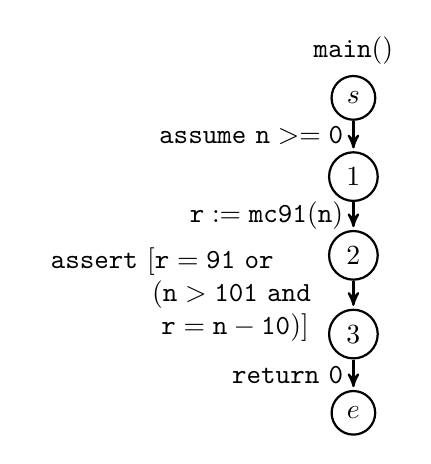
\begin{tikzpicture}[->,>=stealth',shorten >=1pt,auto,node
      distance=2cm,thick,node/.style={circle,draw}]

      \node[node,label=above:$\mathtt{main()}$] (0) at (0, 0)  {$s$};
      \node[node] (1) at (0, -1) {$1$};
      \node[node] (2) at (0, -2) {$2$};
      \node[node] (3) at (0, -3) {$3$};
      \node[node] (4) at (0, -4) {$e$};

      \path
        (0) edge 
            node [left] {$\mathtt{assume\ n >= 0}$} (1)
        (1) edge 
            node [left] {$\mathtt{r := mc91(n)}$} (2)
        (2) edge 
            node [left] {$
              \begin{array}{l}
                \mathtt{assert\ {[}r = 91\ or}\\
                \mathtt{\ \ \ \ \ \ \ \ \ \ \ (n > 101\ and\ \ }\\
                \mathtt{\ \ \ \ \ \ \ \ \ \ \ \ r = n - 10){]}}
              \end{array}$} (3) 
        (3) edge 
            node [left] {$\mathtt{return\ 0}$} (4);
    \end{tikzpicture}

    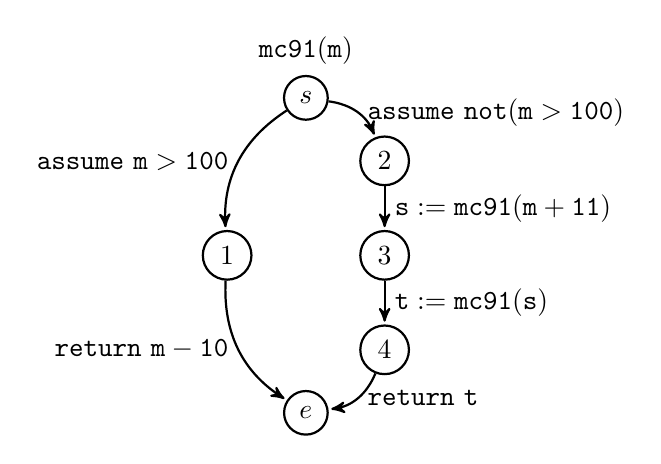
\begin{tikzpicture}[->,>=stealth',shorten >=1pt,auto,node
      distance=2cm,thick,node/.style={circle,draw}]
      \node[node,label=above:$\mathtt{mc91(m)}$] (0) at ( 0,  0) {$s$};
      \node[node] (1) at (-1, -2) {$1$};
      \node[node] (2) at ( 1, -0.8) {$2$};
      \node[node] (3) at ( 1, -2) {$3$};
      \node[node] (4) at ( 1, -3.2) {$4$};
      \node[node] (5) at ( 0, -4) {$e$};

      \path
        (0) edge [bend right=30]
            node [left] {$\mathtt{assume\ m > 100}$} (1)
            edge [bend left=30]
            node [right] {$\mathtt{assume\ not(m > 100)}$} (2)
        (1) edge [bend right=30]
            node [left] {$\mathtt{return\ m - 10}$} (5)
        (2) edge 
            node [right] {$\mathtt{s := mc91(m + 11)}$} (3)
        (3) edge 
            node [right] {$\mathtt{t := mc91(s)}$} (4)
        (4) edge [bend left=30]
            node [right] {$\mathtt{return\ t}$} (5);
    \end{tikzpicture}
  }
  \caption{McCarthy 91 function}
  \label{figure:mccarthy91}
\end{figure}
\end{overlayarea}
\end{frame}

\begin{frame}{Under-approximation of Recursive Call}
  Under-approximate recursive function call
  \begin{itemize}
    \item Use $\mathtt{assume\ false}$
  \end{itemize}

  \begin{figure}
  \centering
  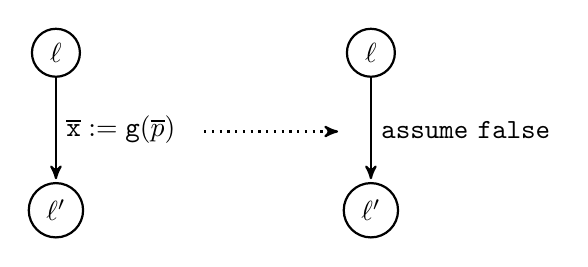
\begin{tikzpicture}[->,>=stealth',shorten >=1pt,auto,node
    distance=2cm,thick,node/.style={circle,draw}]

    \node[node] (0) at (-4, 0)  {$\ell$};
    \node[node] (1) at (-4, -2) {$\ell'$};

    \node[node] (00) at (0, 0)  {$\ell$};
    \node[node] (01) at (0, -2) {$\ell'$};
    \node (arrow_s) at (-2.25, -1) {};
    \node (arrow_e) at (-0.25, -1) {};

    \path
    (arrow_s) edge [dotted] node {} (arrow_e)
    (0) edge 
      node {$\overline{\mathtt{x}} := \mathtt{g} (\overline{p})$}
    (1)

    (00) edge node {$\mathtt{assume\ false}$} (01);
  \end{tikzpicture}
  \end{figure}
  \note {Block some of the execution paths to under-approximate computations}

\end{frame}

\begin{frame}{Under-approximation of Recursive Program}

  Under-approximate recursive program
  \begin{itemize}
    \uncover<2>{\item Replace all recursive calls with $\mathtt{assume\ false}$}
  \end{itemize}

  \begin{figure}
    \tikzstyle{every node}=[font=\small]
    \begin{tikzpicture}[->,>=stealth',shorten >=1pt,auto,node
      distance=2cm,thick,node/.style={circle,draw}]
      \useasboundingbox (-5,-4) rectangle (5,0.5);

      \node[node,label=above:$\mathtt{main()}$] (0) at (0, 0)  {$s$};
      \node[node] (1) at (0, -1) {$1$};
      \node[node] (2) at (0, -2) {$2$};
      \node[node] (3) at (0, -3) {$3$};
      \node[node] (4) at (0, -4) {$e$};

      \path
        (0) edge 
            node [left] {$\mathtt{assume\ n >= 0}$} (1)
        (1) edge 
            node [left]  {\only<2->{\Ccancel[red]}{\color{OliveGreen}$\mathtt{r := mc91(n)}$}} (2)
        (1) edge 
            node [right] {\only<2->{$\color{red}\mathtt{assume\ false}$}} (2)
        (2) edge 
            node [left] {$
              \begin{array}{l}
                \mathtt{assert\ {[}r = 91\ or}\\
                \mathtt{\ \ \ \ \ \ \ \ \ \ \ (n > 101\ and\ \ }\\
                \mathtt{\ \ \ \ \ \ \ \ \ \ \ \ r = n - 10){]}}
              \end{array}$} (3) 
        (3) edge 
            node [left] {$\mathtt{return\ 0}$} (4);
    \end{tikzpicture}
  \end{figure}
\end{frame}

\begin{frame}[fragile]{Transformed C Program}
  \begin{minted}{c}
int main() {
  int n, r;
  assume(n >= 0);

  /* r = mc91(n); */ assume((bool) 0);
  assert(r == 91 || 
    (n>101 && r==n-10));

  return 0;
}
  \end{minted}
\end{frame}

\begin{frame}{More Accurate Approximation}
  
  How to find more accurate under-approximation?
  \begin{itemize}
    \uncover<2->{\item Unwind \uncover<3>{and Replace}}
  \end{itemize}

\begin{overlayarea}{\textwidth}{.6\textheight}
\begin{figure}
  \centering
  \resizebox{\linewidth}{!}
  {  
    \tikzstyle{every node}=[font=\small]
    \begin{tikzpicture}[->,>=stealth',shorten >=1pt,auto,node
      distance=2cm,thick,node/.style={circle,draw}]
      \useasboundingbox (-7.5,-4.5) rectangle (4,0.8);
      
      \node[node,label=above:$\mathtt{main()}$] (0) at (-4, 0) {$s$};
      \node[node] (1) at (-4, -1) {$1$};
      \node[node] (2) at (-4, -2) {$2$};
      \node[node] (3) at (-4, -3) {$3$};
      \node[node] (4) at (-4, -4) {$e$};
    \uncover<2->{
      \node[node] (00) at ( 0,  0){\smallnode{$s_1^{\fun{mc91}}$}};
      \node[node] (01) at (-1, -2) {$1_1$};
      \node[node] (02) at ( 1, -0.8) {$2_1$};
      \node[node] (03) at ( 1, -2) {$3_1$};
      \node[node] (04) at ( 1, -3.2) {$4_1$};
      \node[node] (05) at ( 0, -4) {\smallnode{$e_1^{\fun{mc91}}$}};
    }

      \path
        (0) edge 
            node [left] {$\mathtt{assume\ n >= 0}$} (1)
        (2) edge
            node [left] {$
              \begin{array}{l}
                \mathtt{assert\ {[}r = 91\ or}\\
                \mathtt{\ \ \ \ \ \ \ \ \ \ \ (n > 101\ and\ \ }\\
                \mathtt{\ \ \ \ \ \ \ \ \ \ \ \ r = n - 10){]}}
              \end{array}$} (3) 
        (3) edge 
            node [left] {$\mathtt{return\ 0}$} (4);

      \path
        (1) edge[draw=none] node [left]
          {\color{OliveGreen}{\only<2->{\Ccancel[red]}{$\mathtt{r := mc91(n)}$}}} 
        (2);
    \uncover<1>{
      \path (1) edge (2);
    }
    \uncover<2->{
      \path
        (1) edge [bend left]
            node [above] {$\mathtt{m_1 := n}$} (00)
        (00) edge [bend right]
            node [left] {$\mathtt{assume\ m_1 > 100}$} (01)
            edge [bend left=30]
            node [right] {$\mathtt{assume\ not(m_1 > 100)}$} (02)
        (01) edge [bend right]
            node [left] {$
              \begin{array}{c}
                \mathtt{r^{mc91} :=}\\
                \mathtt{m_1 - 10}
              \end{array}$} (05)
        (02) edge 
            node [right] {
              \only<2>{$\mathtt{s_1 := mc91(m_1 + 11)}$
              }\only<3->{\color{red}$\mathtt{assume\ false}$}
            } (03)
        (03) edge 
            node [right] {
              \only<2>{$\mathtt{t_1 := mc91(s_1)}$
              }\only<3->{\color{red}$\mathtt{assume\ false}$}
            } (04)
        (04) edge [bend left]
            node [right] {$\mathtt{r^{mc91}_1 := t_1}$} (05)

        (05) edge [bend left]
             node [below=8pt] {$\mathtt{r := r^{mc91}_1}$} (2);
    }
    \end{tikzpicture}
  }
  %\caption{Under-approximation of McCarthy 91}
  \label{figure:under-mccarthy91}
\end{figure}
\end{overlayarea}
\end{frame}


\begin{frame}[fragile]{Transformed C Program}

  \begin{columns}[T]
    \begin{column}[T]{.4\linewidth}
      \begin{minted}{c}
int main() {
  int n, r;
  assume(n >= 0);

  /* r = mc91(n); */
  /* Unwind Begin */{
  ...
  }/* Unwind End */
  assert(r == 91 || 
    (n>101 && r==n-10));

  return 0;
}
      \end{minted}
    \end{column}

    \begin{column}[T]{.4\linewidth}
      \begin{minted}{c}
/* Unwind Begin */{
  int r_mc91_1, m_1 = n;
  int s_1, t_1;
  if(m_1 > 100){
    r_mc91_1 = m_1 - 10;
    goto RET_1;
  }/* else */
  assume(0);
  assume(0);
  r_mc91_1 = t_1;
  goto RET_1;
RET_1:;
  r = r_mc91_1;
}/* Unwind End */
      \end{minted}
    \end{column}
  \end{columns}

\end{frame}

\begin{frame}{Much More Accurate Approximation}

  Unwind more times and Replace at last
\begin{figure}
  \centering
  \resizebox{1\textwidth}{!}{
    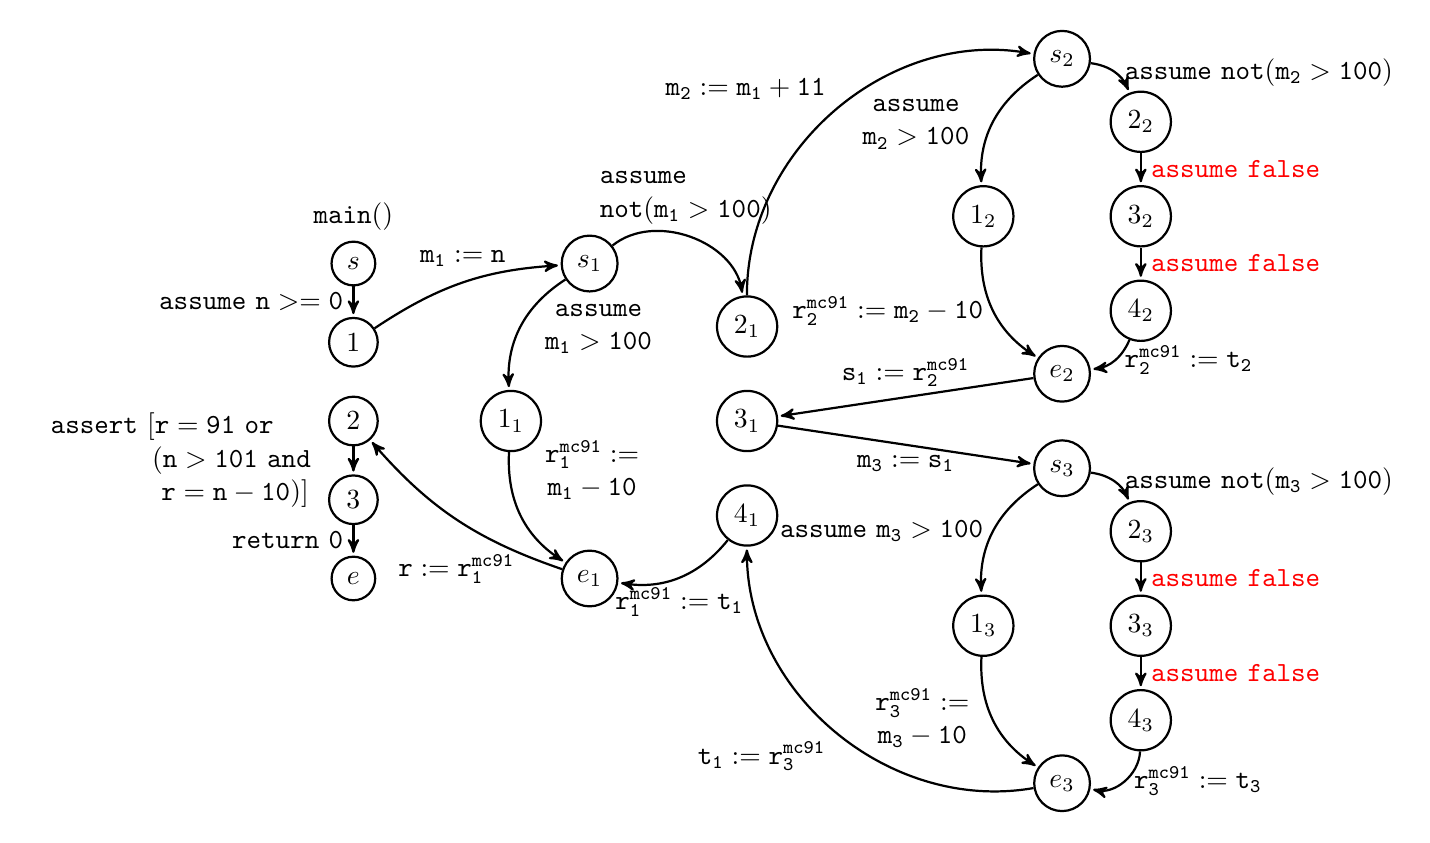
\begin{tikzpicture}[->,>=stealth',shorten >=1pt,auto,node
      distance=2cm,thick,node/.style={circle,draw}]
      \node[node, label=above:$\mathtt{main()}$] (0s) at (-4, 0) {$s$};
      \node[node] (01) at (-4, -1) {$1$};
      \node[node] (02) at (-4, -2) {$2$};
      \node[node] (03) at (-4, -3) {$3$};
      \node[node] (0e) at (-4, -4) {$e$};

      \node[node] (s) at (-1,  0) {$s_1$};
      \node[node] (1) at (-2, -2) {$1_1$};
      \node[node] (2) at ( 1, -0.8) {$2_1$};
      \node[node] (3) at ( 1, -2) {$3_1$};
      \node[node] (4) at ( 1, -3.2) {$4_1$};
      \node[node] (e) at (-1, -4) {$e_1$};

      \node[node] (s') at ( 5,  2.6) {$s_2$};
      \node[node] (1') at ( 4,  0.6) {$1_2$};
      \node[node] (2') at ( 6,  1.8) {$2_2$};
      \node[node] (3') at ( 6,  0.6) {$3_2$};
      \node[node] (4') at ( 6, -0.6) {$4_2$};
      \node[node] (e') at ( 5, -1.4) {$e_2$};

      \node[node] (s'') at ( 5, -2.6) {$s_3$};
      \node[node] (1'') at ( 4, -4.6) {$1_3$};
      \node[node] (2'') at ( 6, -3.4) {$2_3$};
      \node[node] (3'') at ( 6, -4.6) {$3_3$};
      \node[node] (4'') at ( 6, -5.8) {$4_3$};
      \node[node] (e'') at ( 5, -6.6) {$e_3$};

      \path
        (0s) edge 
            node [left] {$\mathtt{assume\ n >= 0}$} (01)
        (01) edge [bend left=15]
            node [above=2pt] {$\mathtt{m_1 := n}$} (s)
        (02) edge 
            node [left] {$
              \begin{array}{l}
                \mathtt{assert\ {[}r = 91\ or}\\
                \mathtt{\ \ \ \ \ \ \ \ \ \ \ (n > 101\ and\ \ }\\
                \mathtt{\ \ \ \ \ \ \ \ \ \ \ \ r = n - 10){]}}
              \end{array}$} (03) 
        (03) edge 
            node [left] {$\mathtt{return\ 0}$} (0e)


        (s) edge [bend right=30]
            node [right] {$
              \begin{array}{c}
                \mathtt{assume}\\ 
                \mathtt{m_1 > 100}                
              \end{array}$} (1)
            edge [bend left=60]
            node [above] {$
              \begin{array}{l}
                \mathtt{assume}\\
                \mathtt{not(m_1 > 100)\ }
              \end{array}$} (2)
        (1) edge [bend right=30]
            node [above right] {$
              \begin{array}{c}
                \mathtt{r^{mc91}_1 :=}\\
                \mathtt{m_1 - 10}
              \end{array}$} (e)
        (2) edge [bend left=50]
            node [above left] {$\mathtt{m_2 := m_1 + 11}$} (s')
        (3) edge 
            node [below] {$\mathtt{m_3 := s_1}$} (s'')
        (4) edge [bend left=30]
            node [below] {$\mathtt{r^{mc91}_1 := t_1}$} (e)
        (e) edge [bend left=15]
            node [below=9pt] {$\mathtt{r := r^{mc91}_1}$} (02)

        (s') edge [bend right=30]
             node [left] {$
               \begin{array}{c}
                 \mathtt{assume}\\
                 \mathtt{m_2 > 100}
               \end{array}$} (1')
             edge [bend left=30]
             node [right] {$\mathtt{assume\ not(m_2 > 100)}$} (2')
        (1') edge [bend right=30]
             node [left] {$\mathtt{r^{mc91}_2 := m_2 - 10}$} (e')
        (2') edge 
             node [right] {\color{red}$\mathtt{assume\ false}$} (3')
        (3') edge 
             node [right] {\color{red}$\mathtt{assume\ false}$} (4')
        (4') edge [bend left=30]
            node [right] {$\mathtt{r^{mc91}_2 := t_2}$} (e')
        (e') edge 
             node [above] {$\mathtt{s_1 := r^{mc91}_2}$} (3)

        (s'') edge [bend right=30]
              node [left] {$\mathtt{assume\ m_3 > 100}$} (1'')
              edge [bend left=30]
              node [right] {$\mathtt{assume\ not(m_3 > 100)}$} (2'')
        (1'') edge [bend right=30]
              node [left] {$
                \begin{array}{c}
                \mathtt{r^{mc91}_3 :=}\\
                \mathtt{m_3 - 10}  
                \end{array}
                $} (e'')
        (2'') edge 
              node [right] {\color{red}$\mathtt{assume\ false}$} (3'')
        (3'') edge 
              node [right] {\color{red}$\mathtt{assume\ false}$} (4'')
        (4'') edge [bend left=50]
              node [right] {$\mathtt{r^{mc91}_3 := t_3}$} (e'')
        (e'') edge [bend left=50]
              node [below left] {$\mathtt{t_1 := r^{mc91}_3}$} (4)
        ;
    \end{tikzpicture}
    }
  %\caption{Unwinding McCarthy 91}
  \label{figure:unwind-mccarthy91}
  \vspace{-1cm}
\end{figure}
\end{frame}


\section{Function Summary with Transformation}
\stepcounter{subsection}

\begin{frame}{Overview}
\tikzstyle{decision} = [diamond, aspect=2, draw, align=center]
\tikzstyle{data} = [draw,trapezium,trapezium left angle=70,trapezium right angle=-70,minimum height=0.6cm]
\tikzstyle{input} = [data, text width=1.7cm]
\tikzstyle{output} = [rounded corners, draw, text width=1.5cm, align=center,minimum height=0.7cm]
\tikzstyle{cross_out} = [red, pos=0.5, auto=false, cross out, -, draw, thick]

\begin{figure}
\begin{tikzpicture}[node distance=1cm and 1.2cm, auto,>=latex', thick]
  % We need to set at bounding box first. Otherwise the diagram
  % will change position for each frame.
  \useasboundingbox (-5.7,-1) rectangle (4.3,4);

  % Nodes
  \node[decision] (analyzer) {Analyzer};
  \node[input, left=of analyzer] (rf_prog) {Intra-proc. Program};

  \node[data, above=.5cm of analyzer,text width=18mm] (proof) {Summary Candidates};

  \node[decision,above=.5cm of proof] (check) {Check};

  \node[input] (rc_prog) at (rf_prog |- check) {Recursive Program};
  \node[output, right=of analyzer] (unsafe) {ERROR};
  \node[output] (safe) at (check -| unsafe) {PASS};

  % Edges
  \path[->]
    (rf_prog) edge (analyzer)
    (analyzer) edge node[anchor=north,sloped]{Error} (unsafe);

  \path[->]
    (rc_prog) edge 
      node[anchor=east]{Under-approx.}
    (rf_prog);

  \path[->]
    (analyzer) edge node[red, anchor=west]{Pass, Compute Summaries} (proof);
  \path[->]
    (proof) edge (check)
    (check) edge node[anchor=south,sloped]{Error, Refine} (rf_prog)
    (check) edge node[anchor=south,sloped]{Pass} (safe);

\end{tikzpicture}
\end{figure}
\end{frame}


\begin{frame}{Over-approximation of Recursive Call}
  Over-approximate recursive function call
  \begin{itemize}
    \item Use $\mathtt{assume}\ S[\mathtt{g}]$
          if $S[\mathtt{g}]$ summarizes the behavior of $\mathtt{g}$
    \item<2-> Derive possible summaries from output of \textsc{BasicAnalyzer}
  \end{itemize}

  \begin{figure}
  \centering
  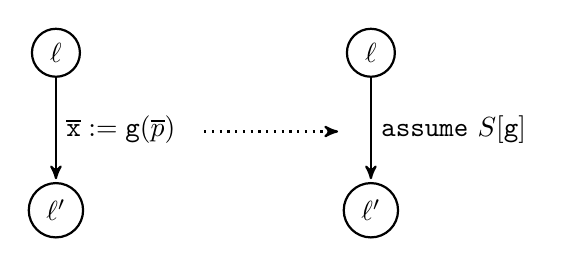
\begin{tikzpicture}[->,>=stealth',shorten >=1pt,auto,node
    distance=2cm,thick,node/.style={circle,draw}]

    \node[node] (0) at (-4, 0)  {$\ell$};
    \node[node] (1) at (-4, -2) {$\ell'$};

    \node[node] (00) at (0, 0)  {$\ell$};
    \node[node] (01) at (0, -2) {$\ell'$};
    \node (arrow_s) at (-2.25, -1) {};
    \node (arrow_e) at (-0.25, -1) {};

    \path
    (arrow_s) edge [dotted] node {} (arrow_e)
    (0) edge
      node {$\overline{\mathtt{x}} := \mathtt{g} (\overline{p})$}
    (1)

    (00) edge node {$\mathtt{assume}\ S[\mathtt{g}]$} (01);
  \end{tikzpicture}
  \end{figure}
  \note {Block some of the execution paths to under-approximate computations}

\end{frame}

\begin{frame}{Desired Program Analyzer}

\begin{overlayarea}{\textwidth}{.12\textheight}
  \textsc{BasicAnalyzer}
  \begin{itemize}
  \item Provide \emph{\alert{inductive invariants}} when program passed analysis
  \end{itemize}
\end{overlayarea}
  \begin{figure}
    \tikzstyle{every node}=[font=\small]
    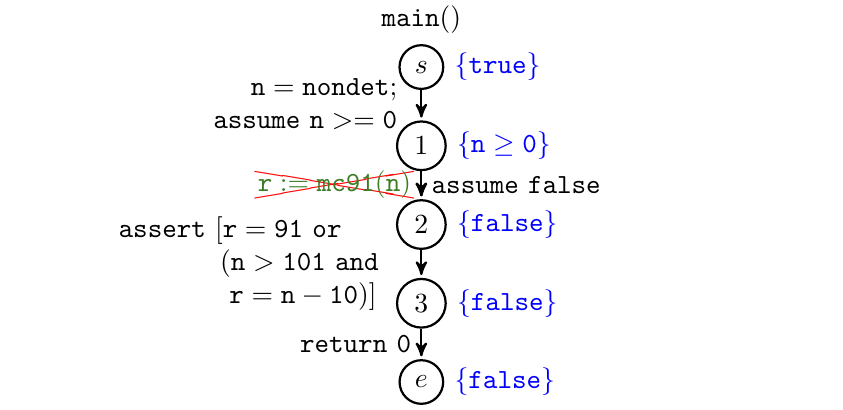
\begin{tikzpicture}[->,>=stealth',shorten >=1pt,auto,node
      distance=2cm,thick,node/.style={circle,draw}]
      \useasboundingbox (-5,-4) rectangle (5,0.5);

      \node[node,label=above:$\mathtt{main()}$] (0) at (0, 0) 
        [label=right:\color{Blue}\{$\mathtt{true}$\}] {$s$};
      \node[node] (1) at (0, -1)
        [label=right:\color{Blue}\{$\mathtt{n \geq 0}$\}] {$1$};
      \node[node] (2) at (0, -2)
        [label=right:\color{Blue}\{$\mathtt{false}$\}] {$2$};
      \node[node] (3) at (0, -3)
        [label=right:\color{Blue}\{$\mathtt{false}$\}] {$3$};
      \node[node] (4) at (0, -4)
        [label=right:\color{Blue}\{$\mathtt{false}$\}] {$e$};

      \path
        (0) edge 
            node [left] {$
              \begin{array}{r}
                \mathtt{n = nondet}; \\
                \mathtt{assume\ n >= 0}
              \end{array}$} (1)
        (1) edge 
            node [left] {\Ccancel[red]{$\color{OliveGreen}{\mathtt{r := mc91(n)}}$}} (2)
        (1) edge
            node [right]{${\mathtt{assume\ false}}$} (2)
                
              
        (2) edge 
            node [left] {$
              \begin{array}{l}
                \mathtt{assert\ {[}r = 91\ or}\\
                \mathtt{\ \ \ \ \ \ \ \ \ \ \ (n > 101\ and\ \ }\\
                \mathtt{\ \ \ \ \ \ \ \ \ \ \ \ r = n - 10){]}}
              \end{array}$} (3) 
        (3) edge 
            node [left] {$\mathtt{return\ 0}$} (4);
    \end{tikzpicture}
  \end{figure}
\end{frame}

\begin{frame}{Compute Function Summaries}

\begin{overlayarea}{\textwidth}{.12\textheight}
  \only<1>{Inductive Invariants for under-approximation
  }\only<2>{Invariants enclose under-approximated function call
  }\only<3>{Extract pair of invariants for function call
  }\only<4>{Replace actual parameters to formal parameters
  }\only<5->{
    Compute with $\mathtt{(\{true\}, \{r^{mc91} \geq 91 \ and\ r^{mc91}=m-10\})}$
  }
  
  \begin{itemize}
    \item {
      \only<1>{Over-approximation of computation of under-approximation
      }\only<2>{Possibly over-approximate original function call
      }\only<3>{$\mathtt{(\{true\}, \{r \geq 91 \ and\ r=n-10\})}$
      }\only<4>{$\mathtt{(\{true\}, \{{\color{BrickRed}r^{mc91}} \geq 91 \ and\ {\color{BrickRed}r^{mc91}}={\color{BrickRed}m}-10\})}$
      }\only<5->{Summary: $\mathtt{true \implies (r^{mc91} \geq 91 \ and\ r^{mc91}=m-10})$}
    }
  \end{itemize}
\end{overlayarea}

\begin{overlayarea}{\textwidth}{.6\textheight}
\begin{figure}
  \centering
  \resizebox{\linewidth}{!}
  {  
    \tikzstyle{every node}=[font=\small]
    \tikzstyle{inv_DC}=[label=right:\color{Blue}\{$\mathtt{...}$\}]
    \begin{tikzpicture}[->,>=stealth',shorten >=1pt,auto,node
      distance=2cm,thick,node/.style={circle,draw}]
      \useasboundingbox (-7.5,-4.5) rectangle (4,0.8);
      
      \node[node,label=above:$\mathtt{main()}$] (0) at (-4, 0)
        [label=left:\color{Blue}\{$\mathtt{true}$\}] {$s$};
      \node[node] (1) at (-4, -1) 
        [label=left:\alt<1>{\color{Blue}}{\color{Red}}\{$\mathtt{true}$\}]
        {$1$};
      \node[node] (2) at (-4, -2) 
        [label=right:\alt<1>{\color{Blue}}{\color{Red}}\scriptsize
          $\begin{Bmatrix}
           \mathtt{r \geq 91 \ and} \\
           \mathtt{r=n-10}
          \end{Bmatrix}$
        ]
        {$2$};
      \node[node, inv_DC] (3) at (-4, -3) {$3$};
      \node[node, inv_DC] (4) at (-4, -4) {$e$};

      \node[node] (00) at ( 0,  0) [label=5:\color{Blue}\{$\mathtt{...}$\}]
        {\smallnode{$s_1^{\fun{mc91}}$}};
      \node[node, inv_DC] (01) at (-1, -2) {$1_1$};
      \node[node, inv_DC] (02) at ( 1, -0.8) {$2_1$};
      \node[node, inv_DC] (03) at ( 1, -2) {$3_1$};
      \node[node, inv_DC] (04) at ( 1, -3.2) {$4_1$};
      \node[node] (05) at ( 0, -4) [label=-5:\color{Blue}\{$\mathtt{...}$\}]
        {\smallnode{$e_1^{\fun{mc91}}$}};

      \path
        (0) edge 
            node [left] {$
              \begin{array}{r}
                \mathtt{n = nondet}; \\
                \mathtt{assume\ n >= 0}
              \end{array}$} (1)
        (2) edge
            node [left] {$
              \begin{array}{l}
                \mathtt{assert\ {[}r = 91\ or}\\
                \mathtt{\ \ \ \ \ \ \ \ \ \ \ (n > 101\ and\ \ }\\
                \mathtt{\ \ \ \ \ \ \ \ \ \ \ \ r = n - 10){]}}
              \end{array}$} (3) 
        (3) edge 
            node [left] {$\mathtt{return\ 0}$} (4);

      \path
        (1) edge[draw=none] node[anchor=center]
          {\color{Gray}{$\mathtt{r := mc91(n)}$}}
        (2);


      \path
        (1) edge [bend left]
            node [above] {$\mathtt{m_1 := n}$} (00)
        (00) edge [bend right]
            node [left] {$\mathtt{assume\ m_1 > 100}$} (01)
            edge [bend left=30]
            node [right] {$\mathtt{assume\ not(m_1 > 100)}$} (02)
        (01) edge [bend right]
            node [left] {$
              \begin{array}{c}
                \mathtt{r^{mc91}_1 :=}\\
                \mathtt{m_1 - 10}
              \end{array}$} (05)
        (02) edge 
            node [right] {$\mathtt{assume\ false}$} (03)
        (03) edge 
            node [right] {$\mathtt{assume\ false}$} (04)
        (04) edge [bend left]
            node [right] {$\mathtt{r^{mc91}_1 := t_1}$} (05)

        (05) edge [bend left]
             node [below=8pt] {$\mathtt{r := r^{mc91}_1}$} (2);

    \uncover<4>{
      \node[node, dashed, left=2.5cm of 0] (decl)
        [label=above:\color{BrickRed}$\mathtt{mc91(m)}$] {$s$};
    }

    \end{tikzpicture}
  }
  \label{figure:inductive-invariants}
\end{figure}
\end{overlayarea}
  \note [figure]{The pair of locations for extract summary is different than described in paper.}
\end{frame}


\begin{frame}{Compute Function Summaries $\sim$}
\begin{itemize}
  \item This method produces summary for one function call
  \item<2-> Function Summary Candidate:\\
            {\color{red}Conjunction} of summaries from {\color{red}marked} function calls
  \item<2-> Details in \S 5.3.
\end{itemize}

\uncover<3->{
\begin{center}
  \Large How to check derived candidates?
\end{center}
}
\end{frame}

\stepcounter{subsection}

\begin{frame}{Overview}
\tikzstyle{decision} = [diamond, aspect=2, draw, align=center]
\tikzstyle{data} = [draw,trapezium,trapezium left angle=70,trapezium right angle=-70,minimum height=0.6cm]
\tikzstyle{input} = [data, text width=1.7cm]
\tikzstyle{output} = [rounded corners, draw, text width=1.5cm, align=center,minimum height=0.7cm]
\tikzstyle{cross_out} = [red, pos=0.5, auto=false, cross out, -, draw, thick]

\begin{figure}
\begin{tikzpicture}[node distance=1cm and 1.2cm, auto,>=latex', thick]
  % We need to set at bounding box first. Otherwise the diagram
  % will change position for each frame.
  \useasboundingbox (-5.7,-1) rectangle (4.3,4);

  % Nodes
  \node[decision] (analyzer) {Analyzer};
  \node[input, left=of analyzer] (rf_prog) {Intra-proc. Program};

  \node[data, above=.5cm of analyzer,text width=18mm] (proof) {Summary Candidates};

  \node[decision,red,above=.5cm of proof] (check) {Check};

  \node[input] (rc_prog) at (rf_prog |- check) {Recursive Program};
  \node[output, right=of analyzer] (unsafe) {ERROR};
  \node[output] (safe) at (check -| unsafe) {PASS};

  % Edges
  \path[->]
    (rf_prog) edge (analyzer)
    (analyzer) edge node[anchor=north,sloped]{Error} (unsafe);

  \path[->]
    (rc_prog) edge 
      node[anchor=east]{Under-approx.}
    (rf_prog);

  \path[->]
    (analyzer) edge node[anchor=west]{Pass, Compute Summaries} (proof);
  \path[->]
    (proof) edge (check)
    (check) edge node[anchor=south,sloped]{Error, Refine} (rf_prog)
    (check) edge node[anchor=south,sloped]{Pass} (safe);

\end{tikzpicture}
\end{figure}
\end{frame}

\begin{frame}{Rough Description for Check}
  \begin{itemize}

  \item Check if candidates over-approximate recursive functions
  \item By Hoare logic proof rule for recursive function
  \begin{itemize}
    \item Given a recursive function and a summary candidate
    \item With assumption that \\
       all recursive calls are summarized by their candidates
    \item Prove its function body is summarized by this candidate
  \end{itemize}
  \item See \S 4.4 and references
  \end{itemize}
\end{frame}

\begin{frame}{Check Function Summaries}

\begin{overlayarea}{\textwidth}{.15\textheight}
  
  Check summary candidate: $\mathtt{r^{mc91} \geq 91 \ and\ r^{mc91}=m-10}$

\uncover<2-> {
  \begin{itemize}
    \item {
      \only<2>{Follow Hoare logic proof rule
      }\only<3>{Replace function call by instantiating the summary
      }\only<4>{Replace $\mathtt{return}$ by assignments to return variables
      }\only<5>{Add an assertion to validate this summary
      }\only<6->{Use \textsc{BasicAnalyzer} to prove this assertion}
    }
  \end{itemize}
}

\end{overlayarea}

\begin{figure}
  \centering
  \resizebox{!}{.45\textheight}
  {
    \alt<6>{\tikzstyle{error_path} = [red]}{\tikzstyle{error_path} = []}
    \begin{tikzpicture}[->,>=stealth',shorten >=1pt,auto,node
      distance=2cm,thick,node/.style={circle,draw}]
      \useasboundingbox (-3.5,-4.5) rectangle (6.5,0.2);

      \node[node,label=above:$\mathtt{mc91(m)}$] (s) at ( 0,  0) {$s$};
      \node[node] (1) at (-1, -2) {$1$};
      \node[node] (2) at ( 1, -0.8) {$2$};
      \node[node] (3) at ( 1, -2) {$3$};
      \node[node] (4) at ( 1, -3.2) {$4$};
      \node[node] (5) at ( 0, -4) {\alt<1-4>{$e$}{$5$}};
      \uncover<5->{\node[node] (e) at ( 0, -5) {$e$};}

      \path
        (s) edge [bend right=30]
            node [left] {$\mathtt{assume\ m > 100}$} (1)
            edge [error_path, bend left=30]
            node [right] {$\mathtt{assume\ not(m > 100)}$} (2)
        (1) edge [bend right=30]
            node [left] {
              \only<1-3>{$\mathtt{return\ m - 10}$
              }\only<4->{\only<4>{\color{red}}$\mathtt{r^{mc91} := m - 10}$}
            } (5)
        (2) edge [error_path]
            node [right] (2_3) {
              \only<1-2>{$\mathtt{s := mc91(m + 11)}$ \only<2>{\color{Blue}{Assume at recursive call}}
              }\only<3->{\only<3>{\color{red}}$
              \begin{array}{l}
              \mathtt{s := nondet;}\\
              \mathtt{assume\ s \geq 91 \ and\ s=m+11-10} 
              \end{array}
              $}
            } (3)
        (3) edge [error_path]
            node [right] (3_4){
              \only<1-2>{$\mathtt{t := mc91(s)}$ \only<2>{\color{Blue}{Assume at recursive call}}
              }\only<3->{\only<3>{\color{red}}$
              \begin{array}{l}
              \mathtt{t := nondet;}\\
              \mathtt{assume\ t \geq 91 \ and\ t=s-10}
              \end{array}$}
            } (4)
        (4) edge [error_path, bend left=30]
            node [right] {
              \only<1-3>{$\mathtt{return\ t}$
              }\only<4->{\only<4>{\color{red}}$\mathtt{r^{mc91} := t}$}
            } (5)
        ;
    \uncover<3>{
      \node [below right=-4mm and 25mm of 2]{\Ccancel[red]{$\mathtt{s := mc91(m + 11)}$}};
      \node [below right=-4mm and 25mm of 3]{\Ccancel[red]{$\mathtt{t := mc91(s)}$}};
    }
    \uncover<2,5->{
      \path
        (5) edge [error_path]
            node [right] (assert) {
              \only<2>  {\color{Blue}{Assert at the exit for proving}
              }\only<5->{\only<5>{\color{red}}$
                \mathtt{assert\ r^{mc91} \geq 91 \ and\ r^{mc91}=m-10}
              $}
            } (e)
        ;}
    \uncover<6->{
      \node [left=4mm of assert]
      {CEX: \color{BrickRed}{$\mathtt{m = 100, r^{mc91}=91}$}};
    }
    \end{tikzpicture}
  }
  %\caption{Check Summary in McCarthy 91}
  \label{figure:check-summary-mccarthy91}
\end{figure}

\end{frame}

\begin{frame}{Check Function Summaries $\sim$}

\begin{overlayarea}{\textwidth}{.15\textheight}
  
  Valid function summary: {$
    \begin{array}{l}
      \mathtt{(m \leq 101\ and\ r^{mc91}=91)\ or} \\
      \mathtt{(m>101\ and\ m-r^{mc91}=10)}
    \end{array}
  $}
\end{overlayarea}

\begin{figure}
  \centering
  \resizebox{!}{.45\textheight}
  {
    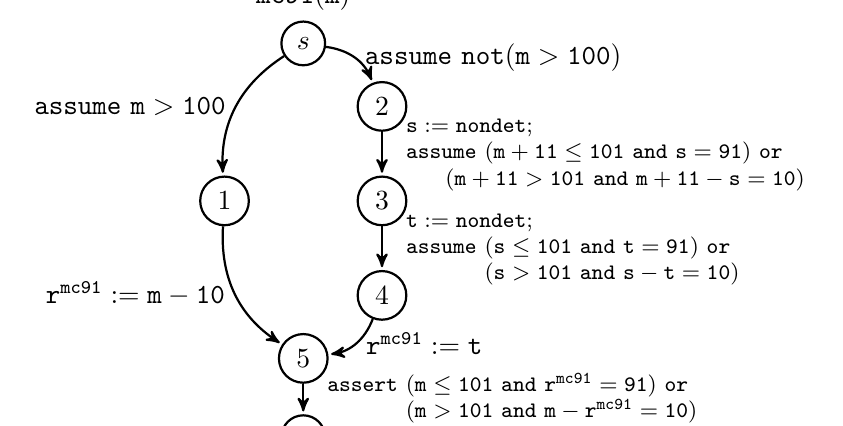
\begin{tikzpicture}[->,>=stealth',shorten >=1pt,auto,node
      distance=2cm,thick,node/.style={circle,draw}]
      \useasboundingbox (-3.5,-4.5) rectangle (6.5,0.2);

      \node[node,label=above:$\mathtt{mc91(m)}$] (s) at ( 0,  0) {$s$};
      \node[node] (1) at (-1, -2) {$1$};
      \node[node] (2) at ( 1, -0.8) {$2$};
      \node[node] (3) at ( 1, -2) {$3$};
      \node[node] (4) at ( 1, -3.2) {$4$};
      \node[node] (5) at ( 0, -4) {$5$};
      \node[node] (e) at ( 0, -5) {$e$};

      \path
        (s) edge [bend right=30]
            node [left] {$\mathtt{assume\ m > 100}$} (1)
            edge [bend left=30]
            node [right] {$\mathtt{assume\ not(m > 100)}$} (2)
        (1) edge [bend right=30]
            node [left] {$\mathtt{r^{mc91} := m - 10}$} (5)
        (2) edge 
            node [right] (2_3) {\footnotesize$
              \begin{array}{l}
                \mathtt{s := nondet;}\\
                \mathtt{assume\ (m+11 \leq 101\ and\ s=91)\ or}\\
                \mathtt{\ \ \ \ \ (m+11>101\ and\ m+11-s=10)}
              \end{array}
            $} (3)
        (3) edge 
            node [right] (3_4){\footnotesize$
              \begin{array}{l}
                \mathtt{t := nondet;}\\
                \mathtt{assume\ (s \leq 101\ and\ t=91)\ or}\\
                \mathtt{\ \ \ \ \ \ \ \ \ \ (s>101\ and\ s-t=10)}
              \end{array}
            $} (4)
        (4) edge [bend left=30]
            node [right] {$\mathtt{r^{mc91} := t}$} (5)
        ;

      \path
        (5) edge
            node [right] (assert) {\footnotesize$
              \begin{array}{l}
                \mathtt{assert\ (m \leq 101\ and\ r^{mc91}=91)\ or}\\
                \mathtt{\ \ \ \ \ \ \ \ \ \ (m>101\ and\ m-r^{mc91}=10)}
              \end{array}
            $} (e)
        ;
    \end{tikzpicture}
  }
  %\caption{Check Summary in McCarthy 91}
\end{figure}

\end{frame}

% TODO
% Add a frame to briefly summarize
\begin{frame}{Overview}
\tikzstyle{decision} = [diamond, aspect=2, draw, align=center]
\tikzstyle{data} = [draw,trapezium,trapezium left angle=70,trapezium right angle=-70,minimum height=0.6cm]
\tikzstyle{input} = [data, text width=1.7cm]
\tikzstyle{output} = [rounded corners, draw, text width=1.5cm, align=center,minimum height=0.7cm]

\begin{figure}
\begin{tikzpicture}[node distance=1cm and 1.2cm, auto,>=latex', thick]
  % We need to set at bounding box first. Otherwise the diagram
  % will change position for each frame.
  \useasboundingbox (-5.7,-1) rectangle (4.3,4);

  % Nodes
  \node[decision] (analyzer) {Analyzer};
  \node[input, left=of analyzer] (rf_prog) {Intra-proc. Program};

  \node[data, above=.5cm of analyzer,text width=18mm] (proof) {Summary Candidates};

  \node[decision,above=.5cm of proof] (check) {Check};

  \node[input] (rc_prog) at (rf_prog |- check) {Recursive Program};
  \node[output, right=of analyzer] (unsafe) {ERROR};
  \node[output] (safe) at (check -| unsafe) {PASS};

  % Edges
  \path[->]
    (rf_prog) edge (analyzer)
    (analyzer) edge node[anchor=north,sloped]{Error} (unsafe);

  \path[->]
    (rc_prog) edge 
      node[anchor=east]{Under-approx.}
    (rf_prog);

  \path[->]
    (analyzer) edge node[anchor=west]{Pass, Compute Summaries} (proof);
  \path[->]
    (proof) edge (check)
    (check) edge node[anchor=south,sloped]{Error, Refine} (rf_prog)
    (check) edge node[anchor=south,sloped]{Pass} (safe);

\end{tikzpicture}
\end{figure}
\end{frame}

\section{Experiments}
\stepcounter{subsection}

\begin{frame}{Implementation}

  {\large \ \ Analyzer for recursive integer program in ANSI C \\}
\begin{itemize}
  \item Algorithm
  \begin{itemize}
    \item Implemented in Python and Objective Caml
    \item About \textbf{2K lines} of code in total
  \end{itemize}

  \item \textsc{BasicAnalyzer}
  \begin{itemize}
    \item \textsc{CPAChecker} 1.2.11-svcomp14b
    \item Won \nth{1} at 2013 and \nth{2} at 2014 in SV-COMP
    \item Over \textbf{140K lines} of Java code
    \item Recursion unsupported
  \end{itemize}

  \item Syntactic transformation for ANSI C program
  \begin{itemize}
    \item CIL~(C Intermediate Language) library
  \end{itemize}

  \item Quantifier Elimination for Linear Integer Arithmetic logic
  \begin{itemize}
    \item \textsc{Redlog}
  \end{itemize}
\end{itemize}
\end{frame}

\begin{frame}{Experiments}

  Benchmarks in 2015 Competition on Software Verification
  \begin{itemize}
    \item \textbf{recursive} category
    \item Total tasks: 24 C programs
    \item Timeout of a task: 900 sec.
  \end{itemize}
  Our tool won \nth{3} Place in the category.

\begin{table}
%\caption{Experimental results of verifying programs in the
%  \textbf{recursive} category of the 2015 Competition on Software
%  Verification.\label{table:experiments}}
\resizebox{\textwidth}{!}
{
\begin{tabular}{|c|cc|c|c|c|c|}
\hline
\multirow{2}{*}{Results} & \multicolumn{2}{c|}{\multirow{2}{*}{Our Tool}} & \textsc{Ultimate} & \textsc{Ultimate} & \multirow{2}{*}{\textsc{SMACK}} & \multirow{2}{*}{\textsc{CPAchecker}} \\ 
& & & \textsc{Automizer} & \textsc{Kojak} & & \\
\hline\hline
correct          & \multicolumn{2}{c|}{12}   & 16  & 8  & 23 & 11 \\ 
false negative   & \multicolumn{2}{c|}{0}    & 0   & 0  & 1  & 0 \\
false positive   & \multicolumn{2}{c|}{0}    & 0   & 0  & 0  & 0 \\
unknown          & \multicolumn{2}{c|}{12}   & 8   & 16 & 0  & 13 \\
\hline\hline
score            & \multicolumn{2}{c|}{\textbf{18}}   & \textbf{25}   & 10  & \textbf{27} & 16 \\
\hline
\end{tabular}
}
\end{table}

\end{frame}


\section{Conclusion}
\stepcounter{subsection}

\begin{frame}{Brief Summary}
  Algorithm
  \begin{itemize}
    \item Use established analyzers as \textsc{BasicAnalyzer}
    \item Enhance \textsc{BasicAnalyzer} via syntactic transformation
  \end{itemize}
  \vfill
  Proof
  \begin{itemize}
    \item Use proof of under-approximation as summary candidates
    \item Verify candidates using Hoare proof rule for recursion  
  \end{itemize}
  \vfill
  Experiment Result
  \begin{itemize}
    \item Our approach is as good as tools specialized for recursion
  \end{itemize}
\end{frame}

\begin{frame}{Advantages}
  Lightweight
  \begin{itemize}
    \item Avoid hacking into \textsc{BasicAnalyzer}
    \item Syntactic transformation only
    \item Much less efforts on implementation
  \end{itemize}
  \vfill
  Modular
  \begin{itemize}
    \item Standard functionality from \textsc{BasicAnalyzer}
    \item Benefit from future advanced analyzers
  \end{itemize}
\end{frame}

%\begin{frame}{Work in progress}
%  Exponential growth of size of transformed program
%  \begin{itemize}
%    \item Due to unwinding recursive calls in each iteration
%    \item Better transformation for analyzers supporting function call
%  \end{itemize}
%  \vfill
%  Participating Competition on Software Verification 2015
%  \begin{itemize}
%    \item \textsc{CPArec} is freely available on GitHub
%    \item \href{https://github.com/fmlab-iis/cparec}{https://github.com/fmlab-iis/cparec}
%  \end{itemize}
%\end{frame}

\begin{frame}{Future Work}

Can this technique handle other kinds of program features, e.g.~Pointer, Concurrency, etc.?

\tikzstyle{decision} = [diamond, aspect=2, draw, align=center]
\tikzstyle{data} = [draw,trapezium,trapezium left angle=70,trapezium right angle=-70,minimum height=0.6cm]
\tikzstyle{input} = [data, text width=1.7cm]
\tikzstyle{output} = [rounded corners, draw, text width=1.5cm, align=center,minimum height=0.7cm]
\tikzstyle{cross_out} = [red, pos=0.5, auto=false, cross out, -, draw, thick]

\begin{figure}
\begin{tikzpicture}[node distance=1cm and 1.2cm, auto,>=latex', thick]
  % We need to set at bounding box first. Otherwise the diagram
  % will change position for each frame.
  \useasboundingbox (-5.7,-1) rectangle (4.3,4);

  % Nodes
  \node[decision] (analyzer) {Analyzer};
  \node[input, left=of analyzer] (rf_prog) {Program w/o feat.};

  \node[input] (rc_prog) at (rf_prog |- check) {Program w/ feat.};

  \node[output, right=of analyzer] (unsafe) {ERROR};
  
  \node[output] (safe) at (check -| unsafe) {PASS};


  % Edges
  \path[->]
    (rf_prog) edge (analyzer)
    (analyzer) edge node[anchor=north,sloped]{Error} (unsafe);
  \path[->]
    (analyzer) edge node[anchor=south,sloped]{Pass} (safe);

  \path[->] (rc_prog) edge node [cross_out]{} (analyzer);

\end{tikzpicture}
\end{figure}

\end{frame}



% Placing a * after \section means it will not show in the
% outline or table of contents.

\begin{frame}

\begin{center}{
  \Huge Thank you $\sim$

\hfill

\hfill 
\includegraphics[width=0.4\textwidth]{img/ASlogoLetterGIF.png}
\hfill 
\includegraphics[width=0.4\textwidth]{img/ntu.png} \hfill
}

\end{center}
\end{frame}

\end{document}


